%%
%% background_and_motivation.tex
\forcecommand{\thesec}{Background}
\section{\thesec}
\label{sec:background_and_motivation}
%%

%%
%% marine icing
\forcecommand{\thesubsec}{Marine Icing}
%%
%% what is your research about? how does it fit into the bigger
%% picture of marine icing research?
\begin{frame}{\thesec}{\thesubsec}
  \vspace*{-3\baselineskip}
  \begin{columns}
    \begin{column}{\paperwidth}
      \begin{figure}
        \centering
        \includestandalone{fig/fig-marine_icing_process}
        \label{fig:marine_icing_process}
      \end{figure}
    \end{column}
  \end{columns}
\end{frame}

%%
%% spray generation
\forcecommand{\thesubsec}{Spray Generation}
%%
\begin{frame}{\thesec}{\thesubsec}
  \vspace*{-0.5\baselineskip}
  \begin{columns}
    \begin{column}{\paperwidth}
      \begin{figure}
        \centering
        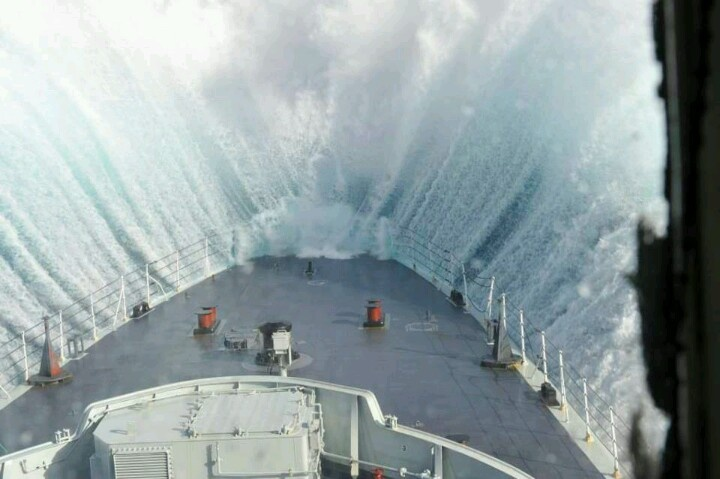
\includegraphics[width=\paperwidth]{img/wave_spray.jpg}
        \label{fig:wave_spray}
      \end{figure}
    \end{column}
  \end{columns}
\end{frame}

\begin{frame}{\thesec}{\thesubsec}
  \vspace*{-\baselineskip}
  \begin{block}{Wave Spray Generation}
    \vspace*{0.5em}
    \begin{itemize}
      \item{
        slamming events produce short-lived bursts of sea spray in a process called \alert{wave spray generation}
      }
      \vspace*{0.5em}
      \item{
        statistical properties of the spray clouds produced following a wave spray event (size distribution of the droplets, velocity distribution, liquid water content) important for prediction of dynamic and thermodynamic behavior of droplets composing spray cloud
      }
    \end{itemize}
  \end{block}
\end{frame}

\begin{frame}{\thesec}{\thesubsec}
  \vspace*{-2\baselineskip}
  \begin{block}{Current Prediction Methods}
    \begin{itemize}
      \item{
        Instead of physical modelling of the spray source, most models of marine icing use empirical equations of spray flux for vessels...and offshore structures (Kulyakhtin, 2014) {\color{white}\cite{Kulyakhtin14}}
      }
      \item{
        empirical formulae require calibration
        \begin{itemize}
          \item{
            performed using data gathered from measurements taken by equipment physically present on a vessel or other structure at sea during spray generation events
          }
        \end{itemize}
      }
      \item{
        calibrated parameters may be appropriately applied to other vessels of similar shape and size, however there is no method by which calibration may be performed for vessels of a novel geometry
        \begin{itemize}
          \item{
            current methods cannot be applied in general!
          }
        \end{itemize}
      }
    \end{itemize}
  \end{block}
\end{frame}
%% M. Sullivan. June, 2016